\documentclass[10pt,twocolumn]{article}

% use the oxycomps style file
\usepackage{oxycomps}

% read references.bib for the bibtex data
\bibliography{references}

% include metadata in the generated pdf file
\pdfinfo{
    /Title (Comps Proposal: \\ Building Self-driving Car With Mindstorms)
    /Author (Maryo Botros)
}

% set the title and author information
\title{Comps Proposal: \\ Building Self-driving Car With Mindstorms}
\author{Maryo Botros}
\affiliation{Occidental College}
\email{mbotros@oxy.edu}

\begin{document}

\maketitle


\section{Introduction and Problem Context}

Robotics boasts a significant benefit in accomplishing repeatable, tedious, or menial tasks at high effieciencies and with great resource utilization. Robots can increase relative productivity and decrease resource and energy consumption by multiple orders of magnitude for processes. They can also offer high-precision with limited human oversight for the tasks they are designed for. The real benefit of robotics comes in where robotics can serve as a substitute for human labor, more specifically, human labor that can potentially put humans in harm's way and some of the best robots for accomplishing this task are vehicles that can navigate autonomously. An example of one of these tasks includes using the robot to enter a building on fire to search for and potentially rescue people. Another application can be for military applications, such as reconnaissance. These are just two of the many possible applications of autonomous vehicles. These robots are very useful, but getting them to accomplish the task of being autonomous does not come easily.

The problem is that getting a robot to navigate any environment is challenging and is rooted in uncertainty. There are two things a robot must be able to do to autonomously navigate. It must understand the map of its environment, which is known as mapping. It must also know where it is on that map, which is known as localization. The problem is that in order for the robot to know where it is on the map, it must first understand the map, but in order for it to understand the map, it must first understand where it is on the map. This poses a major challenge because there are conflicting dependent conditions. The solution to this problem is doing both the mapping and the localization at the same time and this process is known as SLAM. SLAM means simultaneous localization and mapping and it's the method for getting a robot to autonomously navigate its environment. SLAM is still an open problem and new ways of solving the problems of navigation are still being researched constantly.



\section{Technical Background}

A few of the problems involved with navigation that will be covered in this project are localization, searching for the goal location, planning a path to the goal location, covering an entire area, and SLAM.

One of the ways localization is accomplished for robots is using odometry or the distance the robot has traveled. Shaft encoders are the sensors used for odometry. One problem with this however is that the farther the robot has traveled, the more inaccurate the odometry will be because measurements of the physical environment are unavoidable.

Search and path planning involves finding a path from the robot’s current location, to the destination. Two things that the robot would have to know to do this are what the map looks like as well as where it is on that map (localization). It must know both of these within a common frame of reference. There are typically many different paths for getting to the destination from the starting point. Graphs with nodes and lines are usually used for modeling a map. The criterion for the optimal path can be safety or distance for example and finding the optimal path may require searching all paths. A maze is one of the best ways of testing a robot’s ability to get to a goal location. One of the methods for solving a maze can be programming the robot to follow one of the walls of the maze. This method will work but it is the naive solution and is not the most efficient as it can take a long time, depending on the complexity of the maze. A much more optimal solution for solving a maze is by using a depth-first search approach, where the robot will keep track of each path option in the maze as a node and it will go down all the nodes along a single path first before it backtracks and then goes along a different path until it has found the exit to the maze. The way this would be executed is by using a graph data structure, like the one in Figure 1. The graph is a good model for the maze. Each junction in the maze is recorded as a node in the graph model. There are several other algorithms besides the depth-first search for navigating the maze, such as a breadth-first search, but this is one of the most efficient solutions.

Coverage is a problem that certain robots such as robot vacuums need to be able to efficiently solve. If the robot has a map available to it, the problem of coverage becomes a lot easier. In this case, the robot would need all navigable spaces on the map until the whole map is covered, or the robot has accomplished its designated goal, such as searching for an object or reaching a destination. If the robot does not have a map available, there are certain heuristics it can follow such as following a continuous boundary like a wall. 

SLAM is a difficult problem because it requires the robot to do two ongoing processes. One thing that makes SLAM difficult is the data association problem, or basically, the problem that certain locations on the map may look similar, which leads to ambiguity while the robot is navigating. When the robot is constructing a map, if it sees a particular chair at one location and then sees a similar chair at a different location, it would have a hard time distinguishing the two \textcite{Mataric2008TheRoboticsPrimer}.

\begin{figure}
    \centering
    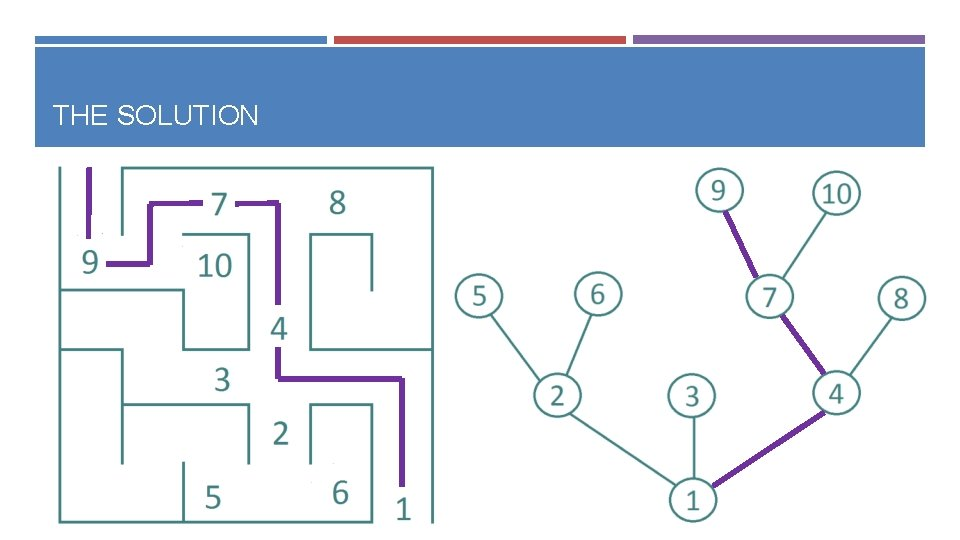
\includegraphics[width=.95\linewidth]{graph.jpg}
    \caption{
        Maze and Graph
    }
    \label{fig:Figure1}
\end{figure}



\section{Prior Work}

As stated earlier, SLAM is still an open problem that is being researched. However, there is already a myriad of already-existing research that sheds light on the greatest advancements in the subject area. Although there are many solutions for solving the problems with SLAM, there are always arising obstacles depending on the application.

In 2018, Geo Week News posted an online article explaining how SLAM is too power-intensive and too slow, which renders it useless for faster robots, such as fast drones. For small drones, SLAM is so power-intensive that there is not enough onboard processing capacity to handle the complex calculations. To combat this issue a new method called NanoMap is being used. Created by researchers at MIT’s Computer Science and Artificial Intelligence Lab (CSAIL), NanoMap uses 3D depth sensors to perform navigation fast, enabling autonomous drones to reach high speeds of up to 20 mph. Unlike SLAM, NanoMap does not generate a holistic map of the environment and uses some uncertainty when it comes to localization. It uses its depth sensors to gather 2D snapshots of its environment and then stores those snapshots. So when it reaches a location, it reaches into its memory and tries to figure out where it is based on how closely related one of the images is to what it is currently seeing \textcite{GeoWeekNewsStaff2018NanoMap}. This is not an ideal approach as there is just too much uncertainty involved, but it does reveal a shortcut that could potentially be useful if it could somehow be combined with SLAM.

Madeline Shiappa, a PhD student at UCF sheds some light on learning methods for SLAM, including the Kalman Filter, which is the most common learning method for SLAM. The Kalman Filter is a type of Bayes Filter used for state estimation It is a recursive algorithm that makes a prediction then goes back and corrects the prediction over time. In order to correct the prediction, sensors are necessary. There are two categories of sensors: proprioceptive and exteroceptive. The exteroceptive sensors are the ones that collect information from the robot’s environment such as if there’s an object in front of the robot and some of these sensors include sonar, range lasers, and cameras. Proprioceptive sensors collect information that is internal to the robot, such as its position and acceleration, using encoders, gyroscopes, and accelerometers. The combination of these two types of sensors produces a very effective feedback system. Madeline Shiappa also acknowledges the computational complexity as a limitation of SLAM. The more dimension in states and measurements, the more intractable the calculations become, which creates a tradeoff between accuracy and complexity \textcite{Schiappa2019HowDoesAutonomous}.



\section{Methods and Evaluation Metrics}

\subsection{Planner}
\subsubsection{Part 1}
The project will be split into three parts. The first is working with a simulation and creating a planner. The second part is building the physical robot using Lego Mindstorms and testing out the planner on the robot. The final part is combining the planner with the use of the robot's sensors to enhance its maze-solving abilities. 

Using a planner will be important for getting the robot to execute its task. The planner I use in this lab will be a hierarchical task network implemented using pyhop. Planning is a key step in preparing a robot to successfully navigate its environment. Planning allows for thoughtful execution for getting from a start state to a goal state without wasting resources such as time and money. For this lab, the task I am looking to achieve is for an agent to navigate a maze using the structure of methods and operators of an HTN (hierarchical task network) planner. I will initialize the start state and goal state in a maze and then program operators and methods to traverse the maze.

To test the effectiveness of the planner code, simulation tests will be run on generated mazes using pyamaze. Since the agent traverses the maze, it requires a path to follow, which stems from converting the resulting plan from the planner code into an actual path for the agent to follow. I will make the planner code a callable function in order to import it. Given the result plan is a dictionary with the directions as the values, I decided with my conversion to a string path, which consists of the 4 cardinal directions (e.g North) as their letter abbreviations (e.g “N” for North”). The simulation runs on these mazes work also in part with assumptions about the maze, such as it being broken down into cells as rows and columns. Of course, the true test is when I implement the planner to path code to the Mindstorms robot to navigate the maze successfully. The approach with the robot is to represent the maze, which is divided into rows and columns that account for the differing size and length of the maze space. This part requires testing just like in the maze simulation to adjust the robot’s velocity and turn values to reach the end of the maze, which there is consideration of utilizing the robot’s sensors to finetune the robot maze navigation.

I will first need to write the operators and methods for the planner using pyhop, in order to get an agent to solve a maze. I will need to use the pyamaze library to generate and solve mazes in simulation. This will allow me to figure out how to solve mazes in a simulated environment without actually working with the robot. Although I will be unable to actually get the robot to solve a maze at this stage, I will learn the general idea of planning for solving a maze

The pyamaze library will allow me to generate mazes such as a 5x5 maze, that specifies coordinates on the maze, which I will refer to as a position on the maze, as well as where the walls are relative to that position. All of this information will be stored in a dictionary of dictionaries, called maze\_map in the pyamaze library.

In Part I, I will start by creating the planner file and importing the pyhop library into it. I also want to keep track of the rows and columns throughout the planner so I will define variables r and c. With that set up, the next step is to come up with the start and goal states.

For the states, I want to keep track of the current position of the agent (coordinates based on the rows and columns), the walls relative to the start position (using maze map, which is a dictionary of dictionaries indicating where the walls are, N,E,S,W, relative to the coordinate on the map), and finally, I want to keep track of whether each of those walls is open or closed (1 indicates open and 0 indicates closed). All of this requires knowing the position of the start and goal states, because if I know the coordinates, I can get all the rest of the information using maze\_map dictionary, which I will call “position\_walls'' in my code. maze\_map has an outer dictionary where the key is the current position. For example, the current position could be (2, 2). The value is another dictionary. The inner dictionary has all the walls as the keys and either a 0 or 1 as the values. An example of an inner dictionary can be {'E': 1, 'W': 0, 'N': 0, 'S': 0}, indicating that all the walls are closed and only the east wall is open, so that is the only viable next direction for the agent. The way I will know the positions of the start state is that the agent always starts out at the bottom right corner, which always has the coordinates of the total number of rows and columns. For example, a three-by-three maze would have a start state position of (3, 3). And the way I know the position of the goal state is that the goal is always at the top left corner of the maze, which will always have the position of (1, 1). Additionally for the start state, I will define the goal (1, 1), as well as a list of all of the positions that the agent has already visited, and a boolean that indicates that the agent has not yet exited the maze:

\begin{verbatim}
    start = pyhop.State('start')
    start.position = (r, c)
    start.walls = position_walls[start.position]
    start.E_wall = position_walls[start.position]['E']
    start.W_wall = position_walls[start.position]['W']
    start.N_wall = position_walls[start.position]['N']
    start.S_wall = position_walls[start.position]['S']
    start.goal = (1, 1)
    start.visited = []
    start.visited.append(start.position)
    start.exit = False
\end{verbatim}

After coming up with the representation, I will work on creating operators and methods for the agent to solve the maze. I will create a task called ‘go’, which has four methods: go\_north, go\_south, go\_east, and go\_west. Each of these methods returns one of four operators if the respective wall is equal to 1 or “open.” The go\_north method for example returns the move\_north operator:

\begin{verbatim}
    def go_north(state, a):
    if state.N_wall == 1:
        return [('move_north', a)]
    else: return False
\end{verbatim}

There are four operators which correspond to the four methods. The operator is what actually updates the location of the agent, and places the visited locations into the visited list. I will do this by keeping track of the current position before the move and calling it prev\_position. I then have to update the row number for the new position and keep the same column number, since we are moving north. And since we are moving north, this would mean that the row number would decrease by one (if we were moving south, the row number would increase by one). If I was looking at the move\_west or move\_east operators, the row number for the new position would remain the same and the column number would change (East: add one, West: subtract one).  Additionally, after the new position has been identified, it would be appended to the list of visited positions, and the walls of the state would be updated, using position\_walls, so that we can know which walls are closed and which walls are open at the new location:

\begin{verbatim}
def move_north(state, a):
if state.N_wall == 1:
    prev_position = state.position
    new_row = prev_position[0] - 1
    col = prev_position[1]
    if (new_row, col) not in state.visited:
        state.position = (new_row, col)
        state.visited.append((new_row, col))
        state.E_wall = 
        position_walls[state.position]['E']
        state.W_wall = 
        position_walls[state.position]['W']
        state.N_wall = 
        position_walls[state.position]['N']
        state.S_wall = 
        position_walls[state.position]['S']
        return state
    else: return False
else: return False
\end{verbatim}

However, this won’t be enough and I will need to create a recursive method called “solve\_maze” that will be part of a new task that I will call “solve.” This new method will check if the row position and column position of the current state are  equal to the coordinates of the goal state and if they aren’t, then the “go” task followed by the “solve” task will be returned. 

\begin{verbatim}
    def solve_maze(state, a):
   if (state.position[0] == state.goal[0]) 
   and (state.position[1] == state.goal[1]):
       return []
   else:
       return [('go', a), ('solve', a)]

pyhop.declare_methods('solve', solve_maze)
\end{verbatim}

\subsubsection{Part 2}
In this section of the lab, I will simulate the maze environment using pyamaze to test the planner (created in Part I) and the execution of this plan for a given maze. Running simulations is a good approach to testing for robotics, as hardware is expensive. Direct testing of a robot risks hardware damage, such is the case if a robot gets damaged due to improper obstacle handling or avoidance. Moreover, computational testing takes time. By testing using simulations prior to testing the actual robot, I avoid wasting time handling hardware errors and other robot malfunctions.

As mentioned, the maze environment used in this project is pyamaze, a library which has methods for creating a maze with many parameters (i.e. dimensions, color, etc….). This library also provides functionality for creating an agent and tracing the agent’s movements in the maze, allowing for dynamic simulation of maze solving given a path (a set of directions specifying movement north, east, south, and west at each cell in the maze). In this project I test the planner on both perfect and imperfect mazes to test the limitations and success of depth first search. By using the planner from Part I and translating this to a path that pyamaze can understand, I am able to use an agent to map and test the accuracy of the paths generated from Part I. In doing so, I test the planner in a simulation environment prior to testing directly on the robot itself.

The goal for this project is to convert the planner method from part 1 into an actual path for the agent to follow in the simulation. Another goal is to then configure the code from part 1 in order to give the agent the appropriate path given a maze.

To move the agent on the maze, I will use the trace\_path method which takes a dictionary as its argument, where the key of the dictionary is the agent itself and the value is the path I want it to take.

To run these simulations, I need to configure the project to access the necessary libraries. I first need to install pyamaze by running pip install pyamaze in the terminal of this project. After this installation is completed, I need to check the version of python for compatibility with pyamaze and change versions if incompatible; the pyamaze library requires the use of python 3.

After successfully installing pyamaze and setting up for its use, I will create my first maze. By default, all pyamaze mazes will be set to be a perfect maze. Perfect mazes, mazes where all cells are accessible and there exists only one solution (path) for navigating from any given cell to the goal cell. Perfect mazes are considerably easier to solve because any cell can be used as the starting point rather than requiring starting from a particular position. Hence, the number of starting positions is more plentiful and the solutions easier to find. There will only be a single correct solution, eliminating the need for comparing the runtimes of different solutions and deciphering the best. The starting point of the maze will always be at the bottom right corner, or the position (n,n) for any n x n maze. To change from generating a perfect maze, I can use the loopPercent parameter to a number less than 100 (corresponding to the percentage). I will import the pyamaze and the planner method. My first maze will be a 10x10 perfect maze generated and saved to a csv with the code:

\begin{verbatim}
from pyamaze import maze, COLOR, agent
from planner import planner

# --------------------
# Initialize maze
r, c = 15, 15
m=maze(r, c)
m.CreateMaze(theme=COLOR.light, 
saveMaze=True)
\end{verbatim}

This saveMaze=True saves the maze as a csv file in the current directory. The starting point of the maze, by default, is the bottom right corner of the maze, or (r, c), where r is the number of rows and c is the number of columns. The agent is, by default, placed at this location. I created an agent with a visible footprint and placed it on the maze at this default location with the code:

\begin{verbatim}
m.tracePath({a:path})

\end{verbatim}

To visualize the movement of this agent, I simply use the trace\_path method. However, to use this method I must convert the plan generated using the pyhop planner I created to a path the trace\_path method can understand. Calling the following function on the planner to generate a path accomplishes this:

\begin{verbatim}
def plan_to_path(plan_list):
path = ''
for plan in plan_list:
    action = plan[0]
    direction = action.split('_')[1][0].upper()
    path += direction
return path
\end{verbatim}

To plan for the maze, I need the maze map. I plan for the maze by retrieving the maze map (called position\_walls here) then getting a plan from this map and converting it to a path:

\begin{verbatim}
    position_walls = m.maze_map

    plan = planner(position_walls, r, c, 1, 1)
    path = plan_to_path(plan)
    
\end{verbatim}

To then execute this path, I use the following code:

\begin{verbatim}
    m.tracePath({a:path})
    m.run()

\end{verbatim}

Next, I will test the planner on imperfect mazes by supplying the argument loopPercent with values less than 100. First, when running with loopPercent=50,  the planner does not always find the shortest path. In fact, it rarely does. This is the product of depth first search. Depth first search will look for a solution, but it doesn’t necessarily need to find the best solution. Once the HTN planner finds a solution, it returns it for the plan. Accordingly, it seldom returns the shortest, or most optimal, path.

Finally, I will create two agents to race to the goal, having them start at different corners of the maze. 

There are a few interesting things to pont out. In the planning code, I wrote methods to move\_north, move\_east, move\_south, and move\_west. I noticed that the order in which I declared these methods affected the outcome of the planner. Since I declared move\_north first, move\_south second, move\_east third, and move\_west lastly, the planner preferred moving north to moving south to moving east to moving west whenever there were choices at a juncture. This caused the agents to have vastly different paths with vastly different optimization success based on their starting positions, as one that could move favorably would get to its goal destination far faster than one which had junctures which caused the planner to prioritize an unfavorable direction.


\section{Ethical Considerations}

Self-driving cars are no longer a science-fiction concept; they are starting to become large areas of research, but at their current stage, they pose many safety risks and are far from the levels of safety and sophistication necessary to have them driving on roads today. There are several ethical considerations regarding self-driving cars on the road. The trolley problem is one of the main ethical concerns that comes to light with the introduction of self-driving cars on the road. This is a classic ethical decision-making scenario, where the autonomous vehicle would be forced to decide between saving the lives of certain individuals. Self-driving cars will also change the way responsibility is assigned in accidents on the road. It becomes challenging to fairly allocate responsibility if a vehicle is driven by a computer. Furthermore, autonomous vehicles will require the collection of extensive sensitive information in order to optimize navigation and this creates the possibility of personal information being misused. Additionally, autonomous vehicles may work best if others share the road use transponders and the use of these transponders will give rise to the same issues concerning privacy as the transponders used in autonomous vehicles. Due to all of these problems autonomous vehicles should not be researched further as they create more problems than solutions. Integrating these machines on the road would involve tremendous investments in vehicles and infrastructure as well as a complete overhaul  in attitudes and behaviors. 

\subsection{The Trolley Problem}
The main ethical conflict with autonomous vehicles involves a decision between prioritizing the interests of passengers (arriving quickly and efficiently) or the interests of the community as a whole (making sure roads are safe for everyone using them)  \cite{AutonomousAccidents}. Utilitarianism is the ethical approach that sides with the community interest and it is “the greatest amount of good for the greatest number of people”  \cite{AutonomousAccidents}. A utilitarian approach to crashes would mean minimizing overall casualties in any manner necessary, including sacrificing the passenger of the autonomous vehicle to save the lives of more pedestrians. This invokes the famous trolley problem, a thought experiment in ethics about a fictional scenario in which an onlooker has the choice to save 5 people in danger of being hit by a trolley, by diverting the trolley to kill just 1 person mmm.  Studies have shown that an overwhelming number of people find this approach to be the most moral; one study in particular concluded that 76\% of people thought it more morally good to sacrifice one passenger to save ten pedestrians than vice versa  \cite{AutonomousAccidents}. On the other hand, the studies also found that participants were more likely to buy an autonomous car programmed to save its own passengers over any number of pedestrians, when offered the hypothetical choice between that and a utilitarian car  \cite{AutonomousAccidents}.

These results reveal that this ethical dilemma is also a social one: everyone wants others to behave in a way that leads to the best global outcome, but they are also hypocritically not motivated to practice that behavior themselves. Additionally, the utilitarian approach to accidents would theoretically save the maximum number of people, but consumers don’t seem to want to buy these vehicles and understandably so because they do not guarantee the safety of the passengers and do not necessarily prioritize the passenger’s safety over the safety of others. “Counterintuitively, this may mean that non-utilitarian AVs would be ethically better, since people would be more likely to buy them, resulting in a greater number of lives saved overall simply by having more autonomous vehicles on the road” \cite{AutonomousAccidents}. Furthermore, a utilitarian approach to crashes does not take into account more complex factors, including the social value of victims, such as their age or ethnicity, and whether it is morally worse to actively kill rather than kill through inaction \cite{AutonomousAccidents}. Any algorithm that makes decisions based on social value would need to be supported by a scale of social value, and obviously, not everyone has the same idea about the relative value of different lives  \cite{AutonomousAccidents}. Would a pregnant woman have more social value than a child, for example? Not only is this a difficult dilemma to solve, but this would also mean that the vehicle would need to implement this sort of decision-making, Autonomous vehicles would have to be able to identify and categorize the people involved in each crash based on social factors that may well not be visible on their person, which is beyond the realm of current sensor technology. Sensors would not be able to detect if a person is a murderer versus a school teacher who has never committed a crime.

Another ethical framework, called the Rights Approach, could be considered the opposite of the Utilitarian Approach. It skews more towards the interests of the individual, which could be the passengers of the autonomous car or each pedestrian on the road. One interpretation of this approach indicates that since the main goal of an autonomous vehicle is to move passengers around safely, the passenger has a right to life  \cite{AutonomousAccidents}. But the lives of everyone should be considered, since the autonomous vehicle manufacturer has decided to make a “dangerous machine” and the passengers have decided to ride in the dangerous machine, they both owe pedestrians a duty of care to safety  \cite{AutonomousAccidents}. Since the passengers already understand the risks associated with riding in an autonomous vehicle, it would be more morally right to prioritize the lives of others on the road since they are not taking that same risk. However, if autonomous vehicle manufacturers programmed their cars this way, consumer interest would likely drop immensely, and since that means fewer autonomous vehicles on the road, this might result in a net loss of life due to more casualties from manned vehicles (same as the drawback to the utilitarian approach)  \cite{AutonomousAccidents}. So, both the Utilitarian Approach and the Rights approach seem to result in the catch-22 that programming autonomous vehicles with the more morally correct approach will end in more loss of life overall due to consumers’ selfish, yet understandable desire to protect themselves above others  \cite{AutonomousAccidents}.

\subsection{Allocating Responsibility}
One of the major ethical dilemmas posed by self-driving cars is the allocation of responsibility. Ideally, self-driving cars should never be involved in any accidents, as that is one of the things they are meant to prevent. However, accidents have occurred because of self-driving car technology and sensors can sometimes be faulty when perceiving the environment, so an accident is always a possibility, and understanding who is responsible for the accident can be an issue. Just about all self-driving cars on the road today require that a driver be in the driver’s seat and this person has just as much responsibility as any other driver on the road. However, this is only a temporary solution as self-driving cars are meant to be completely autonomous and all people in the car will be considered proper passengers. When we reach the point where cars are completely autonomous and the computer processing artificial intelligence is the entity that is “driving,” who is responsible for the safety of the passengers in the car as well as the safety of others traveling and walking on the same roads? Would it be the vehicle owner, vehicle manufacturer, passengers, or someone else?

Two major forms of responsibility can be used to analyze the issues with allocating responsibility when it comes to self-driving cars: task responsibility, commonly referred to as “forwards-looking responsibility,” and blame responsibility, often called “backwards-looking" responsibility. Having a task responsibility means being obliged to do something. Having a blame responsibility means that one is to be blamed if something goes wrong \cite{EthicalOverview}. Blame responsibility is often associated with punishments or with duties to compensate. Our responsibility ascriptions will certainly change when driverless cars are introduced. Users of fully automated vehicles have no control over the vehicle, other than their choice of a destination, so it would be difficult to hold them responsible either for safety (task responsibility) or for accidents (blame responsibility) because we cannot hold people responsible for something they have no control over \cite{EthicalOverview}.

\subsection{Data}
In order for self-driving cars to work effectively, a lot of data needs to be collected and stored such as data from the car’s sensors. This data helps the cars get smarter in a way; as they collect more data, the cars gain a better understanding of their environment and therefore better at navigating the environment. The more data that is collected and processed, the more effective the car will be autonomously driving passengers around. Storing this data can pose some security risks, however, as this data includes the location of the cars and therefore the passenger’s locations. Although this information is vital for the success of the autonomous system, some may consider the collection of this sort of data to be unethical because it can potentially end up in the wrong hands and if it does, it could be detrimental to a person’s identity, finances, and livelihood.

Something else to consider when it comes to the data that is collected by autonomous cars is that the information gathered by the vehicle itself would be complemented by well-developed communication systems, meaning vehicle-to-vehicle communication as well as vehicle-to-road management communications and this would put even more data at risk. Vehicle-to-vehicle communication would allow for Information about obstacles ahead to be obtained before they are registered by the car’s own sensors. Furthermore, sensor or sensor interpretation errors can be detected by comparison with information from other cars or from the roadside \cite{EthicalOverview}. If vehicle-to-road-management systems are interconnected on a large scale, then they can also be used for optimizing the traffic flow because they can provide updated local information on traffic and accessibility.

Handling person-related information and collecting and processing traffic information can give rise to potential privacy intrusions. Currently, private cars do not necessarily leave any electronic traces, but this would change when the number of autonomous vehicles on the road increases as these vehicles will depend on geopositioning transponders and possibly on centralized systems that keep track of each vehicle’s planned route and destination and this information will be linked to the owner and possibly even the passengers \cite{EthicalOverview}.

\subsection{Conclusion}
In conclusion, the introduction of autonomous vehicles on the road gives rise to a plethora of ethical problems. It will change the way in which responsibility ascriptions concerning accidents and traffic safety and responsibility will fall more on the constructors and maintainers of the autonomous vehicles, roads, and their communication systems. Autonomous vehicles will require the collection of extensive sensitive information in order to optimize navigation and this information can be misused. Additionally, autonomous vehicles may work best if others sharing the road use transponders and the use of these transponders will give rise to the same issues concerning privacy as the transponders used in the autonomous vehicles. Because of all of these reasons, it seems to be quite clear that autonomous cars pose too many risks and dangers and the costs far outweigh the benefits. If autonomous vehicles were to be adopted, there would need to be a lot more research conducted in order to address and solve the ethical problems associated with them. 


\section{Timeline}
\begin{itemize}
    \item May 6 - May 22: Complete the HTN Planner
    \item May 23 - June 4: Play with Lego Mindstorms and read documentation
    \item June 5 - June 18: Redo Tutorial and pay closer attention
    \item June 5 - June 18: Redo Tutorial and pay closer attention
    \item June 19 - July 2: Project planning/make fun projects with Mindstorms 
    \item July 3 - July 16: Project planning /make fun projects with Mindstorms 
    \item July 17 - July 30: Project planning/make fun projects with Mindstorms  
    \item July 31 - August 13: Project planning/make fun projects with Arduino 
    \item August 14 - August 27: Build the robot car. 
    \item August 28 - September 10: Begin writing code for the car to navigate the maze using only sensors
    \item September 11 - September 24: Complete writing the code for the car to navigate the maze using only sensors;
    \item September 25 - October 8: Begin integrating the planner with the use of the sensors to make the full self-driving car. 
    \item October 9 - October 22:  Complete integrating the planner with the use of the sensors to make the full self-driving car. 
    \item October 23 - November 5: Iron out any kinks/meet with professors to ask any final questions/begin poster. 
    \item November 6 - November 15: Complete poster
    \item November 16 - December 3: Practice presentation
    \item December 4 - December 15: Place final touches. 

\end{itemize}

\printbibliography

\end{document}
